\documentclass[tikz,border=4mm]{standalone}
\usepackage{amsmath,amssymb}
\usepackage{tikz}
\usetikzlibrary{arrows.meta,positioning,shapes.geometric,shapes.misc,fit,backgrounds,decorations.pathreplacing,shadows,calc}

% Academic Color Palette
\definecolor{seqblue}{RGB}{24, 76, 120}
\definecolor{seqbluebg}{RGB}{242, 247, 252}
\definecolor{lawgreen}{RGB}{22, 101, 52}
\definecolor{lawgreenbg}{RGB}{240, 253, 244}
\definecolor{alertred}{RGB}{190, 18, 60}
\definecolor{alertredbg}{RGB}{255, 241, 242}
\definecolor{amberdark}{RGB}{180, 83, 9}
\definecolor{amberdarkbg}{RGB}{254, 243, 199}
\definecolor{graydark}{RGB}{75, 85, 99}
\definecolor{graydarkbg}{RGB}{243, 244, 246}
\definecolor{boxborder}{RGB}{148, 163, 184}

\begin{document}
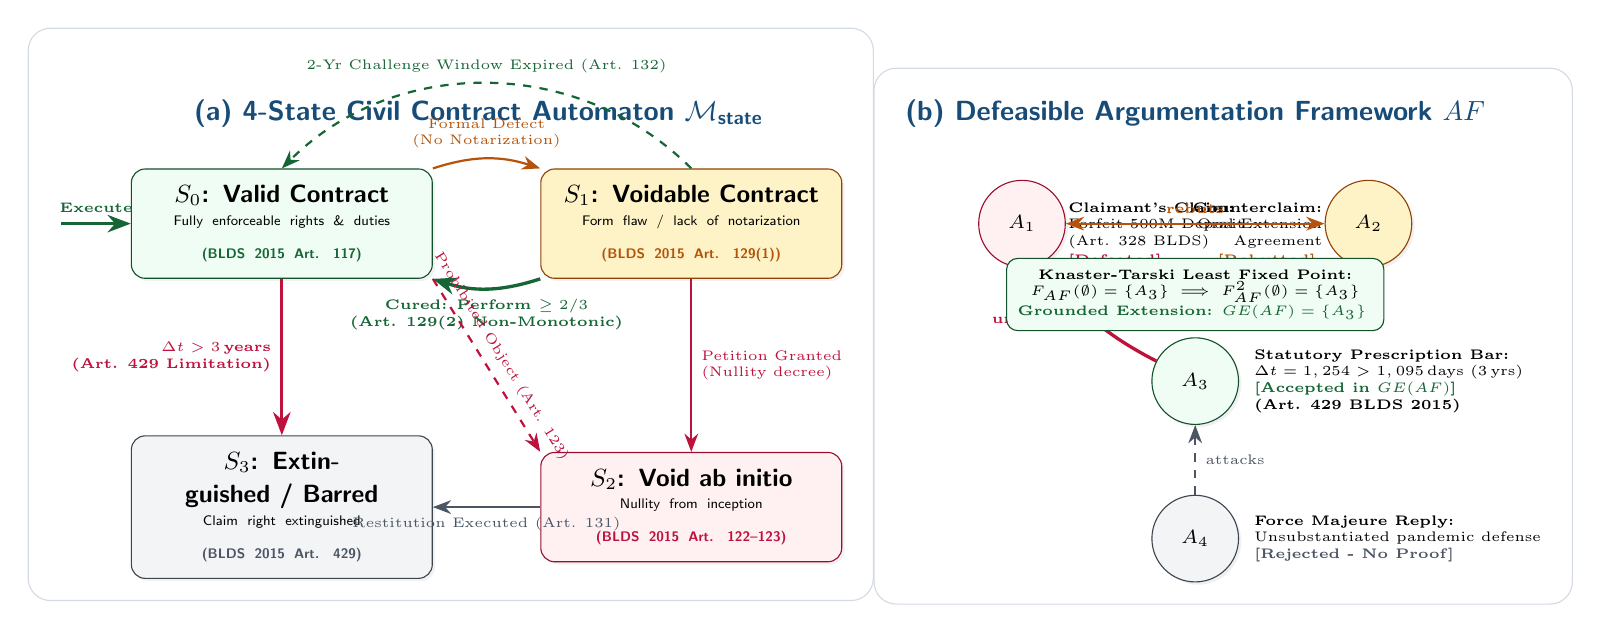
\begin{tikzpicture}[
    font=\sffamily,
    >=Stealth,
    state/.style={
        rectangle,
        rounded corners=5pt,
        draw=#1!80!black,
        fill=#1bg,
        drop shadow={opacity=0.10, shadow xshift=1pt, shadow yshift=-1pt},
        inner sep=6pt,
        text width=3.4cm,
        align=center
    },
    arg/.style={
        circle,
        draw=#1!80!black,
        fill=#1bg,
        drop shadow={opacity=0.12, shadow xshift=1pt, shadow yshift=-1pt},
        inner sep=4pt,
        font=\sffamily\bfseries\scriptsize,
        minimum size=1.1cm,
        align=center
    },
    panel/.style={
        draw=boxborder!60,
        fill=white,
        rounded corners=6pt,
        inner sep=10pt
    }
]

% ==============================================================================
% SUBFIGURE (a): 4-STATE CONTRACT AUTOMATON
% ==============================================================================
\begin{scope}[local bounding box=subfig_a]
    \node[font=\sffamily\bfseries\normalsize, color=seqblue] at (3.5, 3.2) {(a) 4-State Civil Contract Automaton $\mathcal{M}_{\text{state}}$};

    % Initial entry pointer
    \coordinate (start) at (-1.8, 1.8);
    
    % S0: Valid
    \node[state=lawgreen] (S0) at (1.0, 1.8) {
        \textbf{\small $S_0$: Valid Contract}\\[2pt]
        \tiny Fully enforceable rights \& duties\\
        \color{lawgreen}\textbf{(BLDS 2015 Art. 117)}
    };
    \draw[->, very thick, color=lawgreen] (start) -- node[above, font=\tiny\bfseries] {Execute} (S0.west);

    % S1: Voidable
    \node[state=amberdark] (S1) at (6.2, 1.8) {
        \textbf{\small $S_1$: Voidable Contract}\\[2pt]
        \tiny Form flaw / lack of notarization\\
        \color{amberdark}\textbf{(BLDS 2015 Art. 129(1))}
    };

    % S2: Void ab initio
    \node[state=alertred] (S2) at (6.2, -1.8) {
        \textbf{\small $S_2$: Void \textit{ab initio}}\\[2pt]
        \tiny Nullity from inception\\
        \color{alertred}\textbf{(BLDS 2015 Art. 122--123)}
    };

    % S3: Extinguished / Time-Barred
    \node[state=graydark] (S3) at (1.0, -1.8) {
        \textbf{\small $S_3$: Extinguished / Barred}\\[2pt]
        \tiny Claim right extinguished\\
        \color{graydark}\textbf{(BLDS 2015 Art. 429)}
    };

    % Transitions between States
    % S0 -> S1 (Formal flaw discovered)
    \draw[->, thick, color=amberdark] (S0.north east) to[bend left=18] node[above, font=\tiny, align=center] {Formal Defect\\(No Notarization)} (S1.north west);

    % S1 -> S0 (Curing via 2/3 performance Art 129(2)) [CRITICAL SOTA FEATURE]
    \draw[->, very thick, color=lawgreen] (S1.south west) to[bend left=18] node[below, font=\tiny\bfseries, align=center] {\textbf{Cured: Perform $\ge 2/3$}\\\textbf{(Art. 129(2) Non-Monotonic)}} (S0.south east);

    % S1 -> S2 (Court declares void)
    \draw[->, thick, color=alertred] (S1.south) -- node[right, font=\tiny, align=left] {Petition Granted\\(Nullity decree)} (S2.north);

    % S0 -> S2 (Direct void ab initio)
    \draw[->, thick, dashed, color=alertred] (S0.south east) -- node[above, font=\tiny, sloped] {Prohibited Object (Art. 123)} (S2.north west);

    % S0 -> S3 (Prescription bar expired or performance complete)
    \draw[->, very thick, color=alertred] (S0.south) -- node[left, font=\tiny\bfseries, align=right] {$\Delta t > 3$\,years\\(Art. 429 Limitation)} (S3.north);

    % S1 -> S0 (Challenge window expired without suit)
    \draw[->, thick, color=lawgreen, dashed] (S1.north) to[out=135, in=45] node[above, font=\tiny] {2-Yr Challenge Window Expired (Art. 132)} (S0.north);

    % S2 -> S3 (Restitution completed)
    \draw[->, thick, color=graydark] (S2.west) -- node[below, font=\tiny] {Restitution Executed (Art. 131)} (S3.east);
\end{scope}

% ==============================================================================
% SUBFIGURE (b): DEFEASIBLE DUNG ABSTRACT ARGUMENTATION FRAMEWORK
% ==============================================================================
\begin{scope}[xshift=10.2cm, local bounding box=subfig_b]
    \node[font=\sffamily\bfseries\normalsize, color=seqblue] at (2.4, 3.2) {(b) Defeasible Argumentation Framework $AF$};

    % Arguments
    \node[arg=alertred] (A1) at (0.2, 1.8) {$A_1$};
    \node[arg=amberdark] (A2) at (4.6, 1.8) {$A_2$};
    \node[arg=lawgreen] (A3) at (2.4, -0.2) {$A_3$};
    \node[arg=graydark] (A4) at (2.4, -2.2) {$A_4$};

    % Argument Descriptions
    \node[right=2pt of A1.north east, font=\tiny, align=left, anchor=north west] {
        \textbf{Claimant's Claim:}\\
        Forfeit 500M Deposit\\
        (Art. 328 BLDS)\\[1pt]
        \color{alertred}\textbf{[Defeated]}
    };

    \node[left=2pt of A2.north west, font=\tiny, align=right, anchor=north east] {
        \textbf{Counterclaim:}\\
        Oral Extension\\
        Agreement\\[1pt]
        \color{amberdark}\textbf{[Rebutted]}
    };

    \node[right=2pt of A3.east, font=\tiny, align=left, anchor=west] {
        \textbf{Statutory Prescription Bar:}\\
        $\Delta t = 1,254 > 1,095$\,days (3\,yrs)\\
        \color{lawgreen}\textbf{[Accepted in $GE(AF)$]}\\
        \textbf{(Art. 429 BLDS 2015)}
    };

    \node[right=2pt of A4.east, font=\tiny, align=left, anchor=west] {
        \textbf{Force Majeure Reply:}\\
        Unsubstantiated pandemic defense\\
        \color{graydark}\textbf{[Rejected - No Proof]}
    };

    % Defeat and attack relations
    % Mutual attack between A1 and A2
    \draw[<->, thick, color=amberdark] (A1) -- node[above, font=\tiny\bfseries] {rebuts} (A2);

    % Asymmetric defeat from A3 to A1
    \draw[->, very thick, color=alertred, -{Stealth[scale=1.3]}] (A3) to[bend left=15] node[left, font=\tiny\bfseries] {undercuts} (A1);

    % Attempted attack A4 -> A3
    \draw[->, thick, dashed, color=graydark] (A4) -- node[right, font=\tiny] {attacks} (A3);

    % Knaster-Tarski computation summary box
    \node[draw=lawgreen!80!black, fill=lawgreenbg, rounded corners=4pt, inner sep=4pt, font=\tiny, align=center] at (2.4, 0.9) {
        \textbf{Knaster-Tarski Least Fixed Point:}\\
        $F_{AF}(\emptyset) = \{A_3\} \implies F_{AF}^2(\emptyset) = \{A_3\}$\\
        \color{lawgreen}\textbf{Grounded Extension: $GE(AF) = \{A_3\}$}
    };
\end{scope}

% Surrounding boxes for panels
\node[draw=boxborder!40, rounded corners=8pt, fit=(subfig_a), inner sep=8pt] {};
\node[draw=boxborder!40, rounded corners=8pt, fit=(subfig_b), inner sep=8pt] {};

\end{tikzpicture}
\end{document}
